
\subsection{התכנסות הצפיפות והפוטנציאל}
\begin{figure}[h!]
    \begin{minipage}[t]{0.45\textwidth}
        \centering
        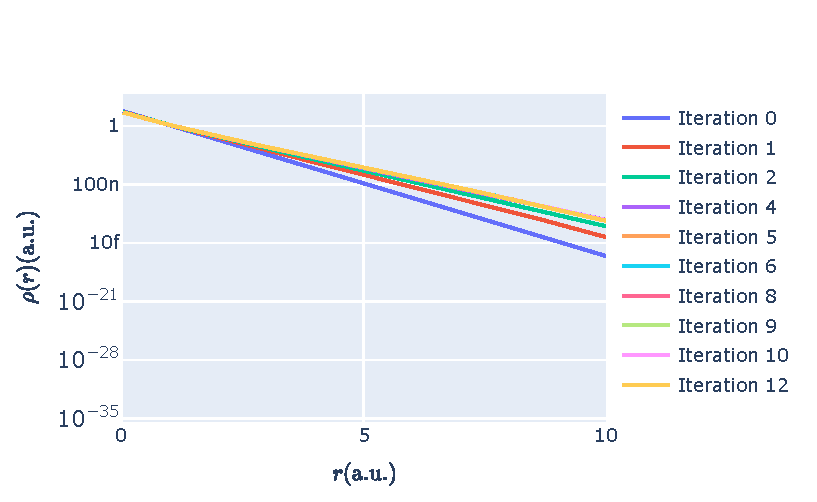
\includegraphics[width=\linewidth, trim=0 0 0 1cm, clip]{plots/helium_atom/electron_density.eps}
        \caption{צפיפות האלקטרונים כתלות ברדיוס עבור האיטרציות השונות. ניתן לראות כי התפלגות האלקטרונים מתרחקת מהראשית - זה מתאים לכוחות הדחיה שפועלים בין האלקטרונים.}
        \label{fig:He_electron_density}
    \end{minipage}
    \hfill
    \begin{minipage}[t]{0.45\textwidth}
        \centering
        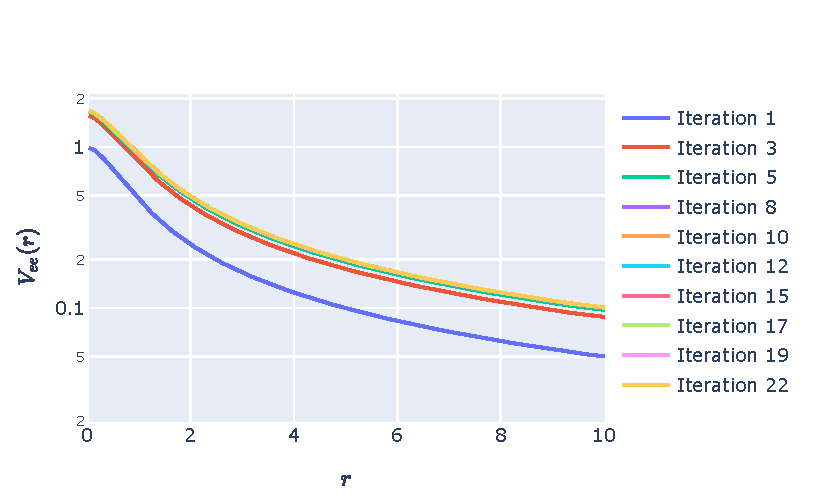
\includegraphics[width=\linewidth, trim=0 0 0 1cm, clip]{plots/helium_atom/electron_electron_potential.eps}
        \caption{הפוטנציאל האלקטרוני כתלות ברדיוס עבור האיטרציות השונות. הפוטנציאל ההתחלתי היה 0 (לא מצוייר) וניתן לראות כי הצורה לא השתנת הרבה לאורך האיטרציות.}
        \label{fig:He_electron_potential}
    \end{minipage}
\end{figure}

התהליך הנומרי התכנס אחרי \input{results/helium_atom/num_iterations} איטרציות, עם טולרנס של $\Delta V_{ee}<10^{-6}$
